\chapter{Self-blindable Credentials\label{chp:self-blindable}}

The drawback of using regular public-key certificates, like X.509
certificates~\cite{ISO9594-8}, is that they are inherently traceable. This is
caused by the fixed public key and the signature that are contained in such a
certificate. The public key can be used as a unique identifier for the user and
is included in the signature, making that identifying as well.

To circumvent this problem Verheul~\cite{Verheul01} proposes a
variant~\cite{BonehLS01,BonehLS04} of the Chaum-Pedersen signature
scheme~\cite{ChaumPedersen93} which allows these values to be randomised, or
\emph{blinded}, such that they are no longer traceable, while the signature can
still be verified for its authenticity. This signature scheme can then be used
to implement a credential system which allows the users themselves to blind
their credentials in order to prevent traceability.

In this chapter we describe the underlying signature schemes and the resulting
credential system as well as our smart card
implementations~\cite{BatinaHJMV10,HoepmanJV10}.

\section{Self-blindable Signatures}

Chaum and Pedersen~\cite{ChaumPedersen93} describe a basic signature scheme
which is intended to be used in combination with smart cards. This scheme
originally operates in the discrete logarithm setting, but is translated to the
elliptic curve setting by Boneh, Lynn and Shacham~\cite{BonehLS01,BonehLS04}
and Verheul~\cite{Verheul01}. The elliptic curve variant of this scheme led to
the construction of self-blindable signatures.

\subsection{Chaum-Pedersen Signature Scheme}

The public key in this scheme is a value $h$ together with a description of the
prime-order group in which the computations take place. As an example we use
$(p, q, g)$, which denotes a subgroup of $\Z^*_p$ of prime-order $q$ with
generator $g$. The corresponding private key is $x = \log_g h$.

\begin{algorithm}[t]
  \caption{Generate a Chaum-Pedersen signature.}
  \label{alg:CP-sign}
  \addtolength{\baselineskip}{1mm}
  \begin{algorithmic}[1]
    \Function{CP-sign}{$m, (p, q, g), x$}
      \State $z \gets m^x \mod p$

      \State $a \gets g^s \mod p$
      \State $b \gets m^s \mod p$

      \State $c \gets \Call{Hash}{m, z, a, b}$

      \State $r \gets s + c \cdot x \mod q$

      \Return $(z, a, b, r)$
    \EndFunction
  \end{algorithmic}
\end{algorithm}

The signature $z$ over a message $m$ is a single exponentiation with the private
key together with a proof that $\log_g h = \log_m z$. This signature can be
generated using Algorithm~\ref{alg:CP-sign}. Verification of the signature
consists of checking the proof according to Algorithm~\ref{alg:CP-verify}. When
the proof is correct, the verifier is assured that the message is signed using
the private key corresponding to the public key used for the verification.

\begin{algorithm}[t]
  \caption{Verify a Chaum-Pedersen signature.}
  \label{alg:CP-verify}
  \addtolength{\baselineskip}{1mm}
  \begin{algorithmic}[1]
    \Function{CP-verify}{$m, (z, a, b, r), (p, q, g), h$}
      \State $c \gets \Call{Hash}{m, z, a, b}$

      \If{$g^r \neq a \cdot h^c \mod p$}
      \Return \Call{Invalid}{}
      \EndIf

      \If{$m^r \neq b \cdot z^c \mod p$}
      \Return \Call{Invalid}{}
      \EndIf

      \Return \Call{Valid}{}
    \EndFunction
  \end{algorithmic}
\end{algorithm}

\subsection{Boneh-Lynn-Shacham Signature Scheme}

Since the signature scheme of Chaum and Pedersen operates in the discrete
logarithm setting it can also be used with elliptic curve cryptography. Boneh,
Lynn and Shacham~\cite{BonehLS01,BonehLS04} present a signature scheme that
works on elliptic curves with bilinear pairings (see Section~\ref{sec:pairings})
and resembles the scheme by Chaum and Pedersen, but omits the equality proof in
order to achieve short signatures.

At the same time Verheul~\cite{Verheul01} gives a similar description of this
proofless variant of the Chaum-Pedersen scheme for groups in which the
decisional Diffie-Hellman problem is easy while the computational Diffie-Hellman
and discrete logarithm problems are hard. Elliptic curves with bilinear pairings
provide such groups. The proof of equality can in this case be substituted by a
bilinear pairing equation to be checked by the verifier.

\begin{algorithm}[t]
  \caption{Generate a Boneh-Lynn-Shacham signature.}
  \label{alg:BLS-sign}
  \addtolength{\baselineskip}{1mm}
  \begin{algorithmic}[1]
    \Function{BLS-sign}{$m, E_1, x$}
      \State $P_m \gets \Call{HashToPoint}{E_1, m}$
      \State $Z \gets x \cdot P_m$

      \Return $Z$
    \EndFunction
  \end{algorithmic}
\end{algorithm}

The public key is a point $Q = x \cdot P_2$ on the elliptic curve $E_2$
together with a description of that curve, of which $P_2$ is the generator. The
private key in this scheme is the scalar value $x$. To sign a message $m$ the
signer transforms it into a point $P_m$ on the curve $E_1$ which is simply
multiplied with the private key as described in Algorithm~\ref{alg:BLS-sign}.

\begin{algorithm}
  \caption{Verify a Boneh-Lynn-Shacham signature.}
  \label{alg:BLS-verify}
  \addtolength{\baselineskip}{1mm}
  \begin{algorithmic}[1]
    \Function{BLS-verify}{$m, Z, E_1, Q$}
      \State $P_m \gets \Call{HashToPoint}{E_1, m}$
      \If{$e(P_m, Q) \neq e(Z, P_2)$}
      \Return \Call{Invalid}{}
      \EndIf

      \Return \Call{Valid}{}
    \EndFunction
  \end{algorithmic}
\end{algorithm}

To verify the signature the verifier has to perform the same check as with the
Chaum-Pedersen scheme, that is, whether the private key used to generate the
signature corresponds to the public key used for the verification. Instead of
using a proof, this can be achieved by checking the following equation (as used
in Algorithm~\ref{alg:BLS-verify}):
\begin{equation}\label{eqn:BLS-verify}
  e(P_m, Q) = e(P_m, x \cdot P_2) = e(x \cdot P_m, P_2) = e(Z, P_2)
\end{equation}
where $e: E_1 \times E_2 \to G$ is a bilinear pairing as described in
Section~\ref{sec:pairings}.

Verheul~\cite{Verheul01} points out a powerful aspect about these signatures:
they are invariant under blinding. When this signature is used to sign points on
the curve,  instead of arbitrary messages, there is no need to transform the
message into a point, such that the \textsc{HashToPoint} operation can be
omitted. Now the user can choose a random number $b$ as blinding factor, and
multiply both the message $P_m$ and signature $Z$ with this factor. The
resulting pair $(b \cdot P_m, b \cdot Z)$ can still be verified using the
verification equation (\ref{eqn:BLS-verify}):
\begin{equation*}
  e(b \cdot P_m, Q)
  = e(b \cdot P_m, x \cdot P_2)
  = e(b \cdot x \cdot P_m, P_2)
  = e(b \cdot Z, P_2)
\end{equation*}
Hence the signature remains valid. Since the user can perform this blinding all
by itself Verheul calls these signatures \emph{self-blindable}.

\section{Verheul's Self-blindable Certificates}

Verheul proposes to use the self-blindable signatures to construct public-key
certificates which allow the user to randomise its key pair and the
corresponding certificate. Such certificates can be used to circumvent
traceability based on the public key or the signature. A certificate of a user's
public key $P_U$ from an identity provider with public verification key $P_{ID}$
takes the form
\begin{equation*}
  \{ P_U, Sig(P_U, s_{ID}) \}\text,
\end{equation*}
where $s_{ID}$ is the private signing key of the identity provider corresponding
to $P_{ID}$.

\subsection{Attribute Certificates}

Attribute certificates are digital certificates that bind attributes to users
known by a public key. Proof of possessing an attribute is given by proving
possession of the private key related to the public key referenced in the
certificate.

$$\{P_U, [Sig(P_U, s_a), Cert(Q_a, \text{"Attribute statement"})]\}$$

Here, the public key $P_U$ of the user is signed using a private key $s_a$ of
the issuer of the attribute. The corresponding public key $Q_a$ of the issuer is
included in a (conventional PKI) certificate which contains the attribute
statement corresponding to this public key. In the context of attribute-based
credentials such a self-blindable attribute certificate can be considered as a
self-blindable credential.

When we consider only a single attribute statement per public key, the
certificates with the statements can be stored in a public database and can be
omitted from the credential, given that the corresponding public key can be
identified. This allows the credentials to be compact which is beneficial for
devices with limited storage capacities, like smart cards.

\begin{figure}[ht]
  \centering
  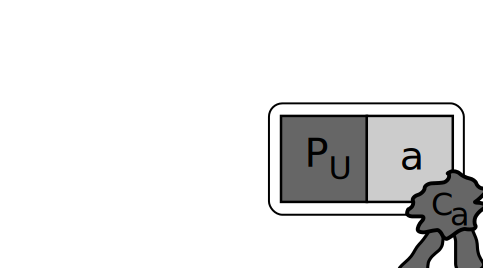
\includegraphics[scale=.45]{images/sbc-credential}
  \caption{A visual representation of a self-blindable credential.}
  \label{fig:SBC-credential}
\end{figure}

\noindent To summarise, a self-blindable credential, as depicted in
Figure~\ref{fig:SBC-credential}, will consist of:
\begin{itemize}
  \item the user's public key $P_U$,
  \item a reference to the attribute statement $a$, and
  \item a signature $C_a = Sig(P_U, s_a) = s_a \cdot P_U$ over the public key
    using the attribute signing key $s_a$.
\end{itemize}
The database will then contain:
\begin{itemize}
  \item a reference $a$,
  \item the public verification key $Q_a$ corresponding to $s_a$, and
  \item the actual attribute statement.
\end{itemize}

\section{Credential Issuance}

\begin{figure}[ht]
  \centering
  \includegraphics[scale=.4]{mscs/sbc_issuance}
  \caption{Issuance of self-blindable credential certificates.}
  \label{fig:SBC-issuance}
\end{figure}

To obtain a self-blindable credential from a credential issuer the user must
provide the issuer with its public key and proof possession of the corresponding
private key. This public key can be signed by an identity provider in order to
increase the trust level of the system. When the credential issuer has verified
the authenticity of the user he will verify eligibility for the requested
attribute. Once this has been verified the issuer signs the user's public key
using the private key corresponding to the requested attribute and send this
signature to the user as depicted in Figure~\ref{fig:SBC-issuance}.

\section{Credential Verification}

When the user wants to utilise an attribute stored in a credential it has to
show the credential to a verifier. To prevent the verifier from tracing her
based on the public key the user first blinds her key pair and the credential as
shown in Figure~\ref{fig:SBC-verification}. Next, she sends the results from
this blinding operation to the verifier and proofs possession of the (blinded)
private key. This last step is easily achieved by signing a challenge received
from the verifier using this private key. The verifier can then verify this
signature using the public key it received earlier.

\begin{figure}[ht]
  \centering
  \includegraphics[scale=.4]{mscs/sbc_verification}
  \caption{Verification of self-blindable credential certificates.}
  \label{fig:SBC-verification}
\end{figure}

\section{Smart Card Implementation}

To understand the practical limitations and estimate the performance of our
protocols, we implemented the protocol from Figure~\ref{fig:SBC-verification}
in Java (for the terminal-side application) and Java Card~\cite{Chen00} (for the
card-side application). Our implementation involves the following components:
\begin{savenotes}
\begin{description}
  \item[Java Card applet\footnote{\url{https://github.com/pimvullers/sbcred_javacard/}
    }\textsuperscript{,}\footnote{An implementation of self-blindable
    credentials for the MULTOS platform is under development at:
    \url{https://github.com/pimvullers/sbcred_multos/}}] ~\\
    The protocol on the card-side is implemented as a Java Card applet and
    loaded onto a development smart card. This implementation will be explained
    in more detail below.

  \item[Bouncy Castle cryptographic library\footnote{\url{http://bouncycastle.org/}}
    with an extension\footnote{\url{https://github.com/pimvullers/bouncycastle-ext/}}\
    for  pairings] ~\\
    The Bouncy Castle library is a collection of
    cryptographic APIs for the C\# and Java programming languages. It provides
    full support for elliptic curve cryptography and an interface to the common
    Java Cryptography Extension API. However, it does not implement pairings or
    elliptic curves over fields other than $\mathbb{F}_p$ and
    $\mathbb{F}_{2^m}$. Thus we have added our own implementations of
    $\mathbb{F}_{p^2}$ and $\mathbb{F}_{p^{12}}$, and the Tate, ate, and R-ate
    pairings.

    This work greatly benefited from an ate pairing in Java that Paulo Barreto
    kindly made available\footnote{\url{https://code.google.com/p/bnpairings/}},
    and algorithms published by Hankerson et al.~\cite{HankersonMS09}. To
    minimise maintenance overhead we strived to keep our extensions purely
    \emph{on top} of the Bouncy Castle library, that is, we did not change
    anything in the original library. This allows for easy integration in newer
    library releases.

  \item[Terminal application\footnote{\url{https://github.com/pimvullers/sbcred_terminal/}}] ~\\
    The protocol on the terminal-side is implemented using the aforementioned
    cryptographic library and the smart card IO library offered by the standard
    Java Development Kit\footnote{Since version 6.0.}. This library offers
    support for communication with smart cards by providing the
    \texttt{javax.smartcardio} package. We used it for the protocol communication
    with the Java Card smart card on which our client applet was installed.
\end{description}
\end{savenotes}

\subsection{Available Elliptic Curve Operations on Java Card}

In order to implement the verification protocol on Java Card we need support for
elliptic curve cryptography. In this section we summarise the operations
available on the Java Card platform and how they can be used to implement the
protocol.

\subsubsection{Elliptic Curve Diffie-Hellman}\label{sec:ecdh-api}

This functionality is provided by the \texttt{javacard.security.KeyAgreement}
class. This class can be instantiated using the \texttt{getInstance()} method
which returns a KeyAgreement object that implements a certain algorithm. The
\texttt{generateSecret()} method can then be used to actually perform the
Diffie-Hellman operation, in our case an elliptic curve multiplication.

The standard Java Card API provides two algorithms~\cite{jcapi222}:
\begin{description}
  \item[]\texttt{ALG\_EC\_SVDP\_DH}: Elliptic curve secret value derivation primitive,
    Diffie-Hellman version, as per IEEE~P1363.
  \item[]\texttt{ALG\_EC\_SVDP\_DHC}: Elliptic curve secret value derivation primitive,
    Diffie-Hellman version, with cofactor multiplication, as
    per IEEE~P1363.
\end{description}
Unfortunately for us, the implementation of these algorithms has two drawbacks:
\begin{enumerate}
  \item According to the IEEE P1363 standard~\cite{IEEE_P1363} the shared
    secret computation by means of ECSVDP-DH and ECSVDP-DHC only returns the
    $x$-coordinate of the computed point.
  \item The Java Card implementation of these algorithms computes the SHA-1
    message digest of the output of the derivation primitive to yield a 20 byte
    result~\cite{jcapi222}.
\end{enumerate}

Especially this last transformation of the point multiplication result prevents
it from being useful for any further computation, other than using it as a
secret key.

\paragraph{JCOP Extension}

Luckily the NXP JCOP platform contains some extensions to the standard Java Card
API. In particular there is an extension which provides an additional algorithm:
\begin{description}
  \item[] \texttt{ALG\_EC\_SVDP\_DH\_PLAIN}: the same as
    \texttt{ALG\_EC\_SVDP\_DH} but without SHA-1 post-computation.
\end{description}
This removes the second drawback as mentioned before and only leaves us with the
$x$-coordinate of the point multiplication result instead of a point. However,
the point can be reconstructed from this coordinate using the elliptic curve
formula. By putting in the $x$ value we can compute the corresponding $y$ value.
The only unknown in this point reconstruction is the sign of the $y$-coordinate,
hence we end up with two candidate points for the multiplication result.

\subsection{Public Key and Credential Blinding}

The first step of the protocol is fairly straightforward. The card has to
select the correct credential for the attribute to reveal and blind it together
with the public key. As described in Algorithm~\ref{alg:SBC-blind} this can be
done by calling the Diffie-Hellman operation once for each value. The resulting
blinded values $P_b$ and $C_b$ are then returned to the terminal.

\begin{algorithm}
  \caption{Public Key and Credential Blinding.}
  \label{alg:SBC-blind}
  \addtolength{\baselineskip}{1mm}
  \begin{algorithmic}[1]
    \Function{SBC-blind}{$b, P_c, C_a$}
      \State $P_b \gets \Call{generateSecret}{P_c, b}$
      \State $C_b \gets \Call{generateSecret}{C_a, b}$

      \Return $P_b, C_b$
    \EndFunction
  \end{algorithmic}
\end{algorithm}

\subsection{Proof of Possession of the Private Key}

Of course, when a terminal receives such a pair $P_b$, $C_b$ it should not only
check that $C_b$ is a proper signature on $P_b$, but also that the card knows
the private key corresponding to the public key $P_b$. This can be done via
standard challenge-response exchange, for example using ECDSA.

\subsubsection{Using the ECDSA Signature Scheme}

As the ECDSA digital signature algorithm is supported by the Java Card API, it
has been our first choice for implementing the challenge-response protocol to
establish proof of possession. As input for this algorithm we need the blinded
private key $k_b = b \cdot k_U$.

Since modular multiplication is not provided by the Java Card API we used the
NatLib library developed by Hendrik Tews~\cite{TewsJacobs09}. This library
implements modular arithmetic on Java Card using basic byte operations as the
RSA operations available on the platform do not support the short values used in
our protocol. The resulting proof of possession protocol is depicted in
Figure~\ref{fig:SBC-proof-ECDSA} and the implementation is described by Batina
et~al.~\cite{BatinaHJMV10}. Unfortunately the use of the NatLib library has an
impact on the performance of the application which made us look into other
alternatives for this protocol.

\begin{figure}[ht]
  \centering
  \includegraphics[scale=.4]{mscs/sbc_proof_ecdsa}
  \caption{Proof of possession of $k_b$ using ECDSA.}
  \label{fig:SBC-proof-ECDSA}
\end{figure}

\subsubsection{Using a minimal variant of the Boneh-Lynn-Shacham Signature Scheme}

\begin{figure}
  \centering
  \includegraphics[scale=.4]{mscs/sbc_proof_bls}
  \caption{Proof of possession of $k_b$ using minimal Boneh-Lynn-Shacham.}
  \label{fig:SBC-proof-BLS}
\end{figure}

Our search led us to, what we denote as, a minimal variant of the
Boneh-Lynn-Shacham signature scheme. Since it consists of only a single point
multiplication using the private key the workload on the card is minimal. We can
also exploit the structure of the message to be signed to reduce the
verification algorithm to a single point multiplication as well. The resulting
proof of possession protocol is depicted in Figure~\ref{fig:SBC-proof-BLS}.

This approach requires us to compute $b \cdot k_U \cdot N$. This can be split
up in two ways, in a modular multiplication and a point multiplication or in two
point multiplications. Since the modular multiplication caused a slow-down in
the previous approach we perform the point multiplications. For this we exploit
the elliptic curve cryptographic key generation functionality\footnote{Using
the Diffie-Hellman operation twice is not an option due to the first drawback
mentioned in Section~\ref{sec:ecdh-api}: the function does not return a point
that can be used for another point multiplication directly, and performing the
point reconstruction on the card would be to costly.} provided by the Java Card
API. This functionality is used to generate the blinding factor and blind the
received challenge at the same time. This allows us to simply sign the blinded
challenge with the private key using the Diffie-Hellman operation, as shown in
Algorithm~\ref{alg:SBC-proof}.

\begin{algorithm}
  \caption{Self-blindable credential verification.}
  \label{alg:SBC-proof}
  \addtolength{\baselineskip}{1mm}
  \begin{algorithmic}[1]
    \Function{SBC-prove}{$P_U, k_U, C_a, N$}
      \State $(b, N_b) \gets \Call{GenerateKey}{N}$
      \State $R \gets \Call{GenerateSecret}{N_b, k_U}$
      \State $P_b \gets \Call{GenerateSecret}{P_U, b}$
      \State $C_b \gets \Call{GenerateSecret}{C_a, b}$

      \Return $P_b, C_b, R$
    \EndFunction
  \end{algorithmic}
\end{algorithm}


\subsection{Terminal Application}

The terminal application needs to cope with the shortcomings of the Java Card
applet. This comes down to the fact that the terminal has to reconstruct the
points $P_b$, $C_b$ and $R$ received from the card before they can be processed
any further.

If we know the $x$-coordinate of a point on the curve, the square of the
corresponding $y$-coordinate is known, namely as $y^{2} = x^{3} + ax + b$.
By taking the square root of $x^{3} + ax + b$ we find either $y$ or $-y$.

This reconstruction is a simple guess work, trying different signs for the
$y$-coordinates of the points. For the proof of possession verification this is
not a real issue since this verification is only a single point multiplication,
although this is of course not optimal. For the pairing signature verification
(\ref{eqn:BLS-verify}) simple guessing is not desirable. Therefore we exploit
the bilinearity of the pairing to avoid computing more than two pairings, as
would be the case without point reconstruction.

First we calculate $e_1 = e(P_b, Q_a)$ and $e_2 = e(C_b, P_2)$ where we take
any sign for the $y$-coordinate of $C_b$. If $e_1 = e_2$, which happens if we
have two right, or two wrong, signs in the first parameters of the pairing, the
verification succeeds. In the remaining case, which means we took one right and
one wrong sign, we check whether $e_1 \cdot e_2 = 1$ holds. If it holds, the
verification also succeeds. This is true because of the following. If
$e_1 \neq e_2$, the error is caused by the wrong sign resulting in one pairing
being the inverse of the other, that is, $e_2 = e_1^{-1}$. Here we can use that
$e_1 \cdot e_2 = e_1 \cdot e_1^{-1} = 1$ to avoid an extra pairing calculation
for the negated point of $C_b$.

\section{Performance Results}

The results of our tests are summarised in Table~\ref{tab:sbc-results}. These
values are the average of ten test runs for each configuration. The table shows
the (accumulated) duration (in milliseconds) of the requests to the card.

\begin{table}[b]
  \centering
  \caption{Test results for various key lengths}
  \label{tab:sbc-results}
  \renewcommand{\tabcolsep}{1.25mm}
  \renewcommand{\arraystretch}{1.25}
  \begin{tabular}{| c || c | c || c |}\hline
    key length & ECDSA & minimal Boneh-Lynn-Shacham & communication \\
    (bits) & (ms) & (ms) & (bytes) \\\hline\hline
    192 & 2748 & 787 & 155 \\\hline
    160 & 1860 & 645 & 135 \\\hline
    128 & 1599 & 535 & 115 \\\hline
  \end{tabular}
\end{table}

When we compare the two implementations it can be seen that the duration of the
ECDSA variant is significantly larger than the minimal Boneh-Lynn-Shacham
solution. This contrast can be explained by the available support from the
cryptographic coprocessor. For the blinding operations in the latter the applet
only uses elliptic curve primitives provided by the coprocessor to perform the
required point multiplications. The blinding in the latter, which requires a
modular multiplication, has to be calculated \emph{without} the help of the
coprocessor.

In theory it is possible to abuse the RSA cipher (and hence use the coprocessor)
to do large part of the modular multiplication by using the fact that
$4ab = (a+b)^2 - (a-b)^2$, as in \cite{Sterckx09,TewsJacobs09}. The squares in
this equation can be performed by doing an RSA encryption\slash exponentiation
with a suitable RSA public key, that is, one with the exponent 2 and the
required modulus. The numbers $a+b$ and $a-b$ are then just messages to be
encrypted using the RSA cipher, which is provided by the Java Card API.

We tried this approach, but unfortunately with no success. The main obstacle is
that the RSA cipher on the card operates only within valid bit lengths for RSA
keys, starting with 512 bit keys. Although the number to be multiplied (the
message) can be any value, the number of non-zero bits in the modulus has to be
at least 488 bits for 512 bit keys according to our tests. Since our modulus is
only 192 bit long the card refused to perform an RSA encryption with such a
short modulus value. However, we believe that a more flexible RSA implementation
on the card would allow this optimisation.

To get some more information about how the running time of the improved
implementation is spent on the card we measured how long it takes to perform the
individual operations. The results of these measurements can be found in
Table~\ref{tab:primitives}. The columns indicate the time needed to perform a
single operation. The processing overhead is determined by subtracting one key
generation and three key agreements from the protocol duration.

\begin{table}
  \centering
  \caption{Test results for the API primitives}
  \label{tab:primitives}
  \renewcommand{\tabcolsep}{1.25mm}
  \renewcommand{\arraystretch}{1.25}
  \begin{tabular}{| c || c | c | c |}\hline
    key length & key generation & key agreement & processing overhead \\
    (bits) & (ms) & (ms) & (ms) \\\hline
    \hline
    192 & 379 & 98 & 114 \\\hline
    160 & 307 & 78 & 104 \\\hline
    128 & 242 & 62 & 107 \\\hline
  \end{tabular}
\end{table}

On the one hand, performing a scalar point multiplication (a key agreement
operation) is quite efficient, using less then 100 milliseconds for the
calculation. On the other hand, performing a scalar point multiplication,
combined with generating a random value, (a key generation operation) is
disappointing, taking more than a factor three longer than just the
multiplication. A possible explanation is a different calculation which explains
the fact that a key generation can return a complete point, whereas a key
agreement can only return the $x$-coordinate.

A large benefit of our use of ECC is the small amount of data that needs to be
exchanged between the terminal and the card. For key lengths of 192, 160 and 128
bits the total amount of bytes exchanged is 155, 135 and 115 respectively. This
would allow an implementation to use a \emph{single} APDU pair (command and
response) for all communication. This is in strong contrast with discrete
logarithm or RSA-based protocols~\cite{Sterckx09,TewsJacobs09} which already
require multiple APDUs to transfer a single command.

%\section{MULTOS implementation??}
%
%On the MULTOS platform the ECC API is also limited to ECDH, ECDSA and key
%generation. We can, however, use the same trick as in the Java Card
%implementation to get the minimal BLS version to work. Furthermore the MULTOS
%API does provide \texttt{ModularMultiplication} operation which allows us to
%efficiently blind the private key, such that we can drop the time consuming key
%generation operation.
%
%[Unfortunately the code does not run.]